Il presente capitolo ha lo scopo di presentare gli strumenti software utilizzati nel corso dello svolgimento del progetto di tesi. Non è obiettivo del capitolo fornire una descrizione esaustiva, la quale è facilmente reperibile da altre fonti, ma darne una'introduzione concisa nell'ottica più ampia del progetto realizzato, specificando allo stesso tempo i motivi che hanno portata a scegliere un determinato strumento software piuttosto che un altro. 
\section{Blender}
Blender è una suite libera e open-source per la creazione di contenuti 3D. Il software supporta l'intero processo produttivo della grafica tridimensionale: modellazione, rigging, animazione, simulazione, rendering, composizione. motion tracking e anche montaggio video.
Blender garantisce un'esperienza coerente su sistemi operativi Linux, macOS e Windows grazie all'utilizzo di OpenGL per l'interfaccia grafica.

Si tratta di uno strumento estremamente versatile, utilizzato in ambiti differenti quali la produzione di animazioni, la creazione di asset per videogiochi, motion graphics, serie televisive, concept art, storyboard, spot pubblicitari e lungometraggi. È impiegato sia da professionisti sia da appassionati e studi di produzione.


\textbf{Caratteristiche principali:}
\begin{itemize}
    \item Blender è una piattaforma completa per la creazione di contenuti 3D, dotata di tutti gli strumenti fondamentali: modellazione, rendering, animazione e rigging, video editing, effetti visivi. compositiong, texture e vari tipi di simulazioni fisiche.
    \item È multipiattaforma, con un'interfaccia grafica basata su OpenGL uniforme su tutti i principali sistemi operativi e può essere personalizzato tramite script Python.
    \item L'architettura interna è progettata per supportare un workflow di produzione rapido ed efficente.
    \item Dispone di una comunità molto attiva e distribuita a livello internazionale, con documentazione, tutoriale risorse disponibili (consultabili, ad esempio, su blender.org/comunity).
    \item Può essere installato ed eseguito da qualsiasi directory senza modificare la configurazione del sistema.
\end{itemize}

\begin{figure}[h]
\begin{center}
     
\includegraphics[width=12cm]{figure/blender.png}
     \caption{Logo del software Blender}
\end{center}
\end{figure}

\subsection{Modellazione, rigging e animazione}
    \begin{itemize}
        \item Modellazione
        
        La modellazione 3D consiste nella creazione della geometria degli oggetti. In Blender questo avviene attraverso la manipolazione di vertici, spigoli (edge) e facce, che insieme formano la mesh.
        Sono disponibili diversi approcci:
        \begin{itemize}
            \item Modellazione poligonale (la più comune): si parte da forme primitive e si raffinano progressivamente con strumenti come estrusione, loop cut e subdivide.
            \item Sculpting: permette una modellazione più organica e fluida, simile alla scultura tradizionale.
            \item Retopologia: processo di semplificazione o ristrutturazione della mesh per renderla più adatta all'animazione.
        \end{itemize}
        L'obiettivo della modellazione, nel contesto dell'animazione, è ottenere una geometria con una topologia pulita, cioè organizzata in modo da deformarsi in maniera controllata quando verrà animata.

        \item Rigging

        Il rigging è il processo di creazione di uno scheletro digitale (armature) che definisce le articolazioni e i punti di movimento dell'oggetto o personaggio.
        L'armatura è costituita da ossa (bones) collegate da relazioni gerarchiche: quando un'osso si muove, i suoi discendenti ereditano la trasformazione.
        Successivamente si definisce tra scheletro e mesh, tramite lo skinning:
        \begin{itemize}
            \item Ogni vertice della mesh viene associato a una o più ossa.
            \item Le influenze delle ossa sui vertici sono rappresentate da pesi (weight painting).
            \item La deformazione della mesh avviene tramite modelli come il Linear Blend Skinning (LBS)
        \end{itemize}
        In sintesi, il rigging stabilisce come l'oggetto potrà muoversi, mentre lo skinning stabilisce come la mesh reagisce a tali movimenti.

        \item Animazione 

        Una volta configurato il rig, è possibile produrre animazione attraverso vari metodi: 
        \begin{itemize}
            \item  KeyFrame Animation: l'animatore definisce manualmente posizioni e pose a istanti temporali specifici, e Blender interpola i movimenti.
            \item Inverse Kinematics (IK): si definisce la posizione finale di una parte del corpo (ad esempio il piede) e il sistema calcola automaticamente le articolazioni intermedie.
            \item Motion Capture/Retargeting: movimenti registrati da attori reali vengono trasferiti allo scheletro.
        \end{itemize}
        Le animazioni sono visualizzate e modificate attraverso strumenti come il \textbf{Dope Sheet}, il \textbf{Graph Editor} e il \textbf{NLA Editor}, che permettono di controllare tempi, curve di interpolazione e combinazione di clip.
    \end{itemize}

\subsection{Strumenti per scripting in Python (bpy)}
Blender integra nativamente un interprete Python e fornisce una API dedicata, denominata bpy, che consente di automatizzare operazioni, creare strumenti personalizzati e interagire con quasi tutti gli elementi presenti nella scena. L'uso di Python rappresenta quindi un modo efficace per estendere a funzionalità del software, ridurre i tempi di lavoro ripetitivi e favorire un workflow riprodubibile.
L'API bpy permette di:
\begin{itemize}
    \item accedere e modificare dati della scena (mesh, materiali, armature, animazioni, ecc.);
    \item eseguire operazioni equivalenti ai comandi della GUI, ma tramite script;
    \item creare operatori personalizzati, pannelli e addon integrabili nell'interfaccia di Blender;
    \item automatizzare pipeline complesse come import/export, rigging, baking o generazione di animazioni.
\end{itemize}
Ad esempio, una mesh può essere letta e modificata tramite codice, i vertex group possono essere manipolati, opppure è possibile controllare direttamente i keyframe di un'animazione. Blender salva inoltre tutte le azioni dell'utente in forma di comandi Python visualizzabili dalla Python Console o dall'Info Log, facilitando l'apprendimento della corrispondenza tra operazioni manuali e comandi programmabili.
L'impiego della scripting API è particolarmente utile quando si lavora con retargeting dell'animazione o generazione procedurale, come nel caso dell'auto-rigging o del trasferimento automatico dei pesi (skinning), poichè consente di operare in modo coerente su più modelli in modo ripetibile e senza intervento manuale.


\section{Mixamo}
Mixamo è una piattaforma online fornita da Adobe che mette a disposizione una vasta libreria di animazioni umanoidi pronte all'uso, progettato per essere applicate direttamente a modelli 3D dotati di rigging scheletrico. La libreria comprende migliaia di movimenti categorizzati per tipologia, come camminate, corse, salti, espressioni corporee, azioni sportive, movimenti stilizzati e animazioni di combattimento. Ogni animazione è creata a partire da dati di motion capture, garantendo una riproduzione realistica della dinamica del movimento umano.
Le animazioni sono inoltre parametrizzabili: l'utente può modificare aspetti quali ampiezza dei gesti, velocità, posizione del baricentro o intensità dell'azione direttamente dell'interfaccia del servizio. Questo rende possibile adattare rapidamente un'animazione alle esigenze specifiche del personaggio o della scena, senza necessità di interventi manuali sull'intero ciclo animato.
Un aspetto rilevante è la compatibilità con rig unamoidi standardizzati, come l'armatura "Mixamo Skeleton". Grazie a questo formato, le animazioni possono essere trasferite con facilità a una vasta gamma di modelli 3D, riducendo la necessità di procedure di retargeting complesse. Inoltre, Mixamo offre uno strumento di auto-rigging che consentono di generare automaticamente lo scheletro del personaggio e assegnare i pesi di skinning, partendo da una semplice mesh umanoide.


\begin{figure}[h]
\begin{center}
     
\includegraphics[width=11cm]{figure/mixamo.jpg}
     \caption{Logo del software Mixamo}
\end{center}
\end{figure}

\subsection{Esportazione in formato FBX e compatibilità con Blender e Unity}
Mixamo consente l'esportazione di modelli riggati e animazioni principalmente nel formato FBX (FilmBox), uno dei formati più diffusi nell'ambito della grafica 3D e dei motori di gioco. Il formato FBX conserva tutte le informazioni necessarie per la riproduzione del movimento, inclusi:
\begin{itemize}
    \item la gerarchia scheletrica (armatura)
    \item i pesi di skinning (associazione vertice-osso)
    \item le curve di animazione relative alla rotazione, traslazione e scala dei giunti.
\end{itemize}
\begin{figure}[H]
        \begin{center}
         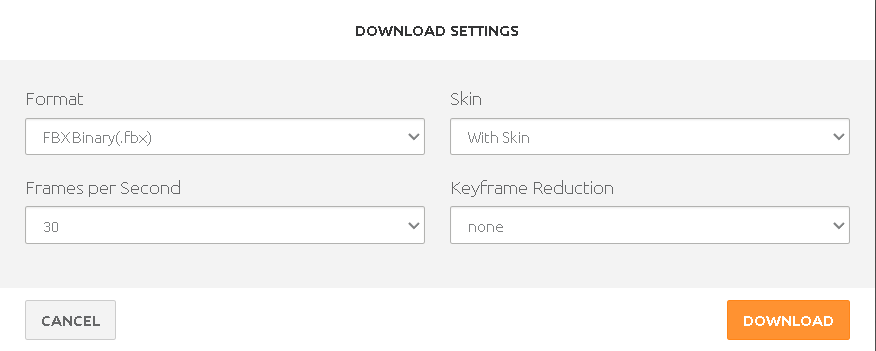
\includegraphics[width=10cm]{figure/fbx.png}
         \caption{Impostazioni per il download delle animazioni}
         \label{fig:fbx}
        \end{center}
    \end{figure}
Queste caratteristica rende l'FBX particolarmente adatto all'interscambio tra software differenti, cosentendo un flusso di lavoro fluido tra Mixamo -> Blender -> Unity.

\medskip
\noindent\textbf{Compatibilità con Blender}\medskip

All'interno di Blender, l'importazione del file FBX mantiene nella maggior parte dei casi:
\begin{itemize}
    \item la struttura dello scheletro Mixamo ("mixamorig"),
    \item le animazioni applicate all'armatura,
    \item la corretta deformazione della mesh durante il movimento.
\end{itemize}
Tuttavia, può essere necessario eseguire alcuni passaggi di adattamento, come:
\begin{itemize}
    \item la normalizzazione delle scale globali,
    \item la riconversione degli assi di orientamento,
    \item la rinominazione automatica dei bones per compatibilità con rig controllers (ad esempio, Rigify).
\end{itemize}
Blender fornisce strumenti per la gestione dell'animazione, tra cui NLA Editor e Dope Sheet, che permettono di combinare, modificare o rifinire le animazioni importate da Mixamo.

\medskip
\noindent\textbf{Compatibilità con Unity} \medskip

Nel motore di gioco Unity, i file FBX importati da Mixamo vengono riconosciuti come Humanoid Rig tramite il sistema di retargeting dell'engine. Questo consente:
\begin{itemize}
    \item l'associazione dei movimenti a personaggi differenti purchè abbiamo un rig umanoide compatibile,
    \item l'utilizzo delle animazione all'interno dello Animator Controller,
    \item la sincronizzazione delle sequenze tramite lo state machine di Unity
\end{itemize}
Inoltre, Unity consente di:
\begin{itemize}
    \item miscelare animazioni (blending),
    \item applicare inverse kinematics in runtime,
    \item creare animazioni procedurali combinate a quelle keyframed.
\end{itemize}
Questo rende l'integrazione delle animazioni Mixamo particolarmente efficace nel contesto della produzione di videogiochi, simulazioni interattive e applicazioni VR/AR.


\section{MoveAI}
MoveAI è un'innovatica piattaforma di motion capture basata sull'intelligenza artificiale che converte video ordinari in animazioni 3D di alta qualità, senza bisogno di marcatori, tute o costose configurazioni. Progettata per creatori di ogni livello, MoveAI utilizza la visione artificiale e l'apprendimento automatico per analizzare il movimento umano, fornendo dati di animazione accurati e realistici direttamente da riprese con una o più telecamere. Grazie a strumenti intuitivi come MoveOne a a prezzi flessibili basati sui crediti, MoveAI consenti a singoli artisti, studi e aziende di creare motion capture di livello professionale a una frazione dei costi tradizionali.


\begin{figure}[H]
\begin{center}
     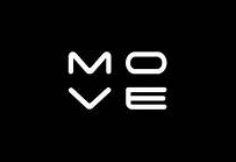
\includegraphics[width=8cm]{figure/move.png}
     \caption{Logo del software MoveAI}
\end{center}
\end{figure}


\subsection{Generazione automatica di animazioni realistiche da video (MoveAI)}
Negli ultimi anni, l'evoluzione dei metodi di motion capture non marked-based ha permesso di ottenere animazioni di qualità cinematografica a partire da semplici video, senza la necessità di tute sensorizzate o sistemi ottici complessi. Tra le tecnologie più avanzate in questo ambito si colloca MoveAI, una piattaforma che utilizza algoritmi di visione artificiale e machine learning per estrarre il movimento umano in modo accurato da sequenze video provenienti anche da più camere commerciali.
MoveAI si basa su una pipeline di elaborazione che integra:
\begin{itemize}
    \item stima della posa 2D in ciascun frame del video;
    \item ricostruzione tridimensionale della posa mediante triangolazione multi-camera;
    \item filtraggio temporale per garantire coerenza a fluidità del movimento;
    \item retargeting automatico del movimento su un modello umanoide virtuale.
\end{itemize}
Il risultato è un'animazione naturalistica e continua, che rispetta ritmo, velocità, dinamica e stile di movimento originale. A differenza dei sistemi tradizionali di motion capture, che richiedono ambienti controllati e strumentazione costosa, MoveAI consente di registrare l'azione in contesti quotidiani, riducento drasticamente i costi di produzione e rendendo più accessibile la creazione di animazioni realistiche.
Sul piano applicativo, questa tecnologia si rivela particolarmente utile in:
\begin{itemize}
    \item animazione 3D e produzione cinematografica,
    \item sviluppo di videogiochi e esperienze immersive,
    \item sport e analisi del movimento,
    \item realtà virtuale e aumentata.
\end{itemize}
Inoltre, l'output generato può essere esportato direttamente come file FBX, consentendo l'integrazione fluida con software come Blender, Maya, Unity, Unreal Engine, e facilitando il retargeting su personaggi diversi attraverso rig umanoidi standard (come mixamorig o Unity Humanoid Rig).

\section{Unity 3D}
Unity è un motore grafico multipiattaforma sviluppato da Unity Technologies che consente lo sviluppo di videogiochi e altri contenuti interattivi, quali visualizzazioni architettoniche o animazioni 3D in tempo reale. L'ambiente di sviluppo Unity gira sia su Microsoft Windows sia su macOS e sia su Linux, e i giochi che produce possono essere eseguiti su Microsoft Windows, macOS, Linux, Xbox 360, PlayStation 3, PlayStation Vita, Wii, iPad, iPhone, Android, Windows Mobile, PlayStation 4, Xbox One, Wii U e Nintendo Switch. Unity consente di utilizzare sia un editor per lo sviluppo/progettazione di contenuti sia un motore di gioco per l'esecuzione del prodotto finale. Unity è simile a Director, Blender Game Engine, Virtools, Torque Game Builder e GameStudio, è inoltre possibile utilizzare un ambiente grafico integrato come metodo primario di sviluppo.

\begin{figure}[H] 
    \begin{center} 
        
\includegraphics[width=10cm]{figure/unity.png} 
        \caption{Logo del software Unity3D} 
    \end{center} 
\end{figure}

\subsection{Gestione dei modelli animati in Unity}
Unity offre un sistema integrato per la gestione di modelli 3D animati, basato sul concetto di Animator, che consente di controllare e riprodurre animazioni in modo dinamico all'interno di una scena interattiva. Una volta importato un modello, Unity riconosce automaticamente la presenza di uno scheletro e associa un rig di animazione configurabile (Figura ~\ref{fig:confi}) in tre modalità: \textbf{Generic}, per personaggi senza struttura umanoide; \textbf{Humanoid}, per modelli con anatomia umana standard; e \textbf{Legacy}, per animazioni basate su clip non scheletriche. L'utilizzo del rig Humanoid è particolarmente vantaggioso, poiché permette di sfruttare la retargeting map interna di Unity, consentendo così la riutilizzabilità delle animazioni tra personaggi differenti.

\begin{figure}[H] 
    \begin{center} 
        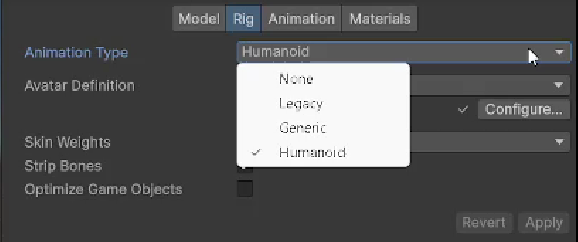
\includegraphics[width=10cm]{figure/confi.png} 
        \caption{Impostazione animazione su Unity} 
        \label{fig:confi}
    \end{center} 
\end{figure}

\subsection{Pipeline di importazione FBX -> Unity}
Il formato FBX rappresenta lo standard più comune per trasferire modelli animati da software di authoring 3D (come Blender o  Maya) verso Unity. Durante l'importazione, Unity applica automaticamente una serie di conversioni, tra cui la normalizzazione delle scale, l'interpretazione dello scheletro e la suddivisione di eventuali clip di animazione contenute nel file.
Una volta importato, il modello può essere configurato tramite l'Inspector: è possibile definire il tipo di rig, controllare a coerenza della gerarchia scheletrica e, se necessario, correggere le pose di riferimento (T-Pose/ A-Pose). L'animazione può quindi essere associata al personaggio attraverso componenti Animator o Animation.

\subsection{Sitema di retargeting delle animazioni: Animator Controller}
Il cuore del sistema di animazione in Unity è l'Animator Controller, uno strumento che consente di definire come e quando un personaggio esegue determinate animazioni. L'Animator Controller funziona tramite una struttura a \textbf{state machine}, dove ogni stato rappresenta una clip di animazione o una combinazione di esse. Le transizioni tra gli stati possono essere controllate da parametri, variabili che vengono aggiornate in tempo reale dal codice o dall'interazione dell'utente.

Quando si utilizza un rig di tipo Humanoid, Unity applica automaticamente il motion retargeting , ovvero la conversione dei movimenti da una sorgente (ad esempio un'animazione proveniente da Mixamo o MoveAI) al modello in scena. Questo processo presenza l'intenzione del movimento, adattandolo alle proporzioni del personaggio, permettendo così di riutilizzare la stessa animazione su avatar differenti senza ulteriori modifiche.